% Appendix A. Instalacion de gnuradio
%==========================================================================

%TODO: Actializar la informacion de instalacion apuntando a la version 3.3.0. Quitar referencias de git
\chapter{Instalaci\'on del ambiente de desarrollo}
\label{AppA}

El desarrollo de aplicaciones basadas en \emph{GNURadio} en el ambiente Linux es m\'as sencillo y m\'as vers\'atil ya que la
mayor\'ia de las librer\'ias externas de las que depende esta herramienta fueron desarrolladas para Linux.
Aunque \emph{GNURadio} proporciona soporte parcial/total para otros sistemas operativos como \emph{Windows} y \emph{Mac OSX}, el
experimento se realiz\'o en el sistema operativo \emph{Ubuntu}, que es una distribuci\'on del sistema operativo
Linux basada en \emph{Debian}. Se opt\'o por esta versi\'on de Linux ya que es amigable y f\'acil de usar pero principalmente se
escogi\'o por su habilidad de poder ser instalado dentro de \emph{Windows} como una aplicaci\'on normal. Esto evita tener que
hacer una partici\'on separada para instalar el sistema operativo. Si se desea quitar es solo cuestion de ir al panel de control
de \emph{Windows} y desinstalar \emph{Ubuntu}. Estar\'a en la lista de aplicaciones instaladas.

Para llevar a cabo este procedimiento se utiliz\'o un programa especial llamado \emph{Wubi} \cite{russo}. Esta aplicaci\'on
instala el sistema operativo dentro de un solo archivo y agrega una nueva opci\'on al men\'u de arranque de la PC para
seleccionarlo aparte del sistema operativo primario. Cuando se ejecuta el programa \emph{Wubi}, se deben especificar las opciones
que se muestran en la figura \ref{fig:wubi}. Se puede dejar el tama\~no del archivo generado en su opci\'on por defecto pero se
recomienda que m\'inimo se le asigne 10 gigabytes para tener suficiente espacio para la instalaci\'on de librer\'ias. Se debe
especificar un nombre de usuario y la clave para esta cuenta ya que ser\'a la cuenta principal donde se realizar\'a todo el trabajo.

\begin{figure}[hpt]
\centering
	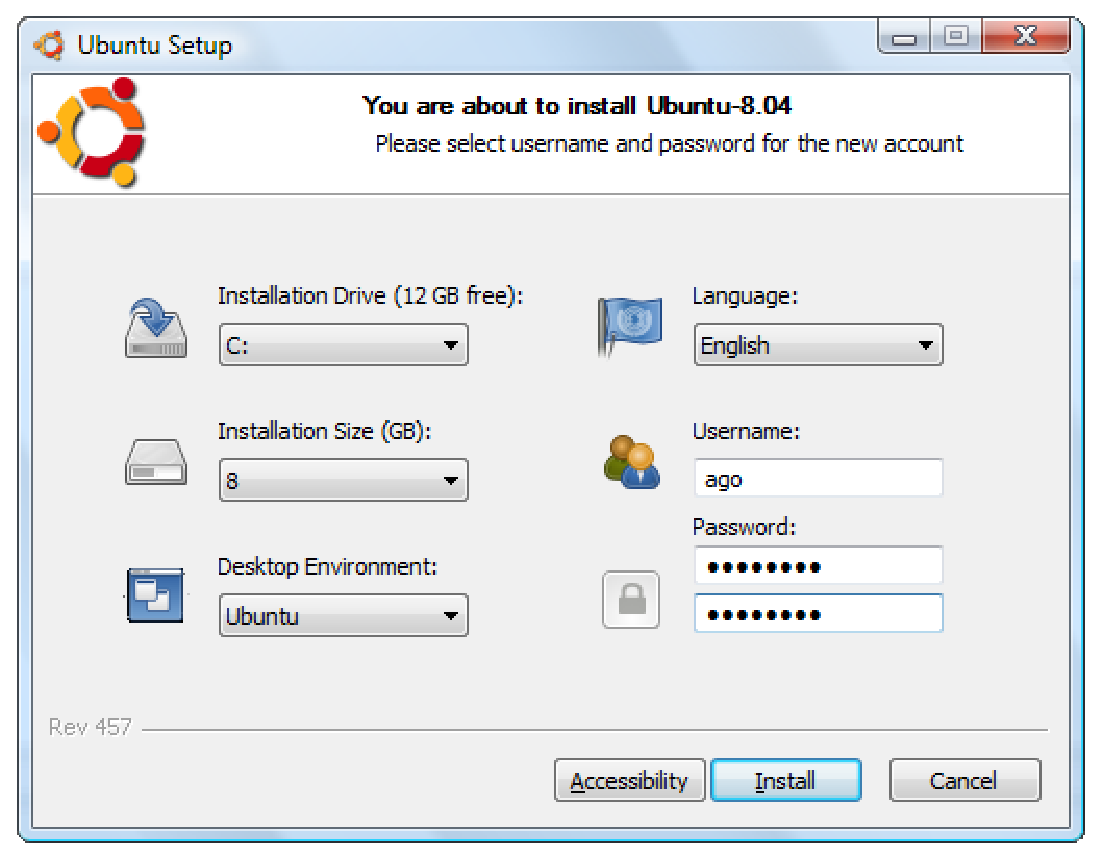
\includegraphics[scale=0.5]{figs/wubi}
	\vspace{0.1in}
	\caption{Opciones del instalador \emph{Wubi}}
	\label{fig:wubi}
\end{figure}

Una vez que se halla especificado las opciones anteriores se puede iniciar con la instalaci\'on. \emph{Wubi} comenzar\'a a
descarga la imagen del DVD correspondiente a la distribuci\'on de \emph{Ubuntu} que se especific\'o.

Cabe mencionar que la instalaci\'on puede ser de 32 o 64 bits, dependiendo del
tipo de instalaci\'on de \emph{Windows} en que se instalar\'a \emph{Ubuntu}. Si
el sistema operativo principal es de 32 bits entonces la instalaci\'on tambi\'en
ser\'a de 32 bits. Esto se debe tener presente cuando se inicie la instalaci\'on
de \emph{GNURadio} ya que las librer\'ias de las cuales depende vienen en
versiones de 32 y 64 bits.

La imagen mide aproximadamente 700MB. Cuando termine la descarga la aplicaci\'on
comenzar\'a a crear el archivo del sistema operativo y agregar\'a la opci\'on para
seleccionarlo en el men\'u de arranque como se muestra en la figura
\ref{fig:bootmenu}. Una vez terminado este procedimiento la aplicaci\'on le
pedir\'a al usuario que reinicie la PC. Se debe seleccionar la nueva opci\'on del men\'u
de arranque para ingresar al sistema operativo \emph{Ubuntu}. Al terminar se le presentar\'a al usuario que ingrese el
nombre de la cuenta y la clave. Esta es la que se especific\'o en el instalador
\emph{Wubi}. Al ingresar se presenta el escritorio \emph{GNOME} (o \emph{KDE} si se especific\'o otra distribuci\'on como
\emph{Kubuntu}) como se muestra en la figura \ref{fig:desktop}.

\begin{figure}[htp]
\centering
	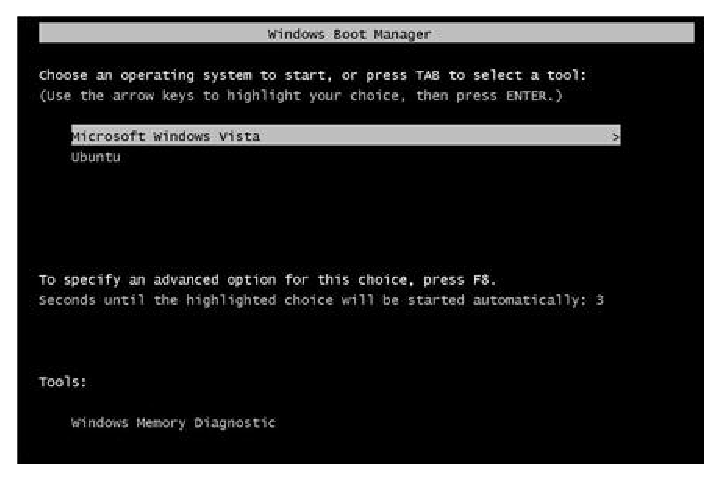
\includegraphics[scale=0.8]{figs/boot}
	\vspace{0.1in}
	\caption{Men\'u de arranque con la opci\'on de \emph{Ubuntu}}
	\label{fig:bootmenu}
\end{figure}

\begin{figure}[htp]
\centering
	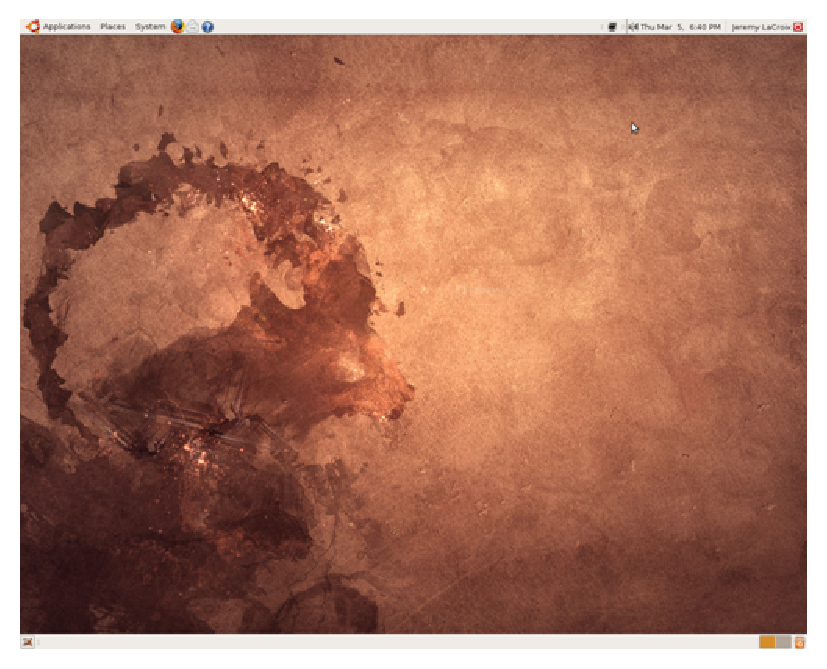
\includegraphics[scale=0.7]{figs/desk}
	\vspace{0.1in}
	\caption{Escritorio \emph{GNOME} de la distribuci\'on \emph{Ubuntu}}
	\label{fig:desktop}
\end{figure}

El siguiente paso es instalar \emph{GNURadio} y sus dependencias. Todas las dependencias se pueden conseguir utilizando el sistema
de instalaci\'on de software de \emph{Ubuntu}. Utilizando el sistema Synaptic del sistema operativo se deben instalar las
dependencias que se especifican en la tabla \ref{tbl:radioreqs}.

\begin{table}[htp]
\begin{center}
	\begin{tabular}{|p{6cm}|p{7.5cm}|}
		\hline
		Tipo & Elementos \\
		\hline
		Herramientas de desarrollo que se requieren para compilar el c\'odigo fuente.
		& 
		\begin{itemize}
		  \item g++
		  \item subversion
		  \item make
		  \item autoconf, automake, libtool
		  \item sdcc
		  \item guile
		  \item ccache
		  \item SWIG 1.3.31 o mayor
		  \item git
		\end{itemize} \\
		\hline
		Librer\'ias requeridas para compilaci\'on y funcionamiento de los ejecutables.
		&
		\begin{itemize}
		  \item python-dev
		  \item FFTW 3.X (fftw3, fftw3-dev)
		  \item CppUnit (libcppunit y libcppunit-dev)
		  \item Boost 1.35 o mayor
		  \item libusb y libusb-dev
		  \item wxWidgets (wx-common y python-wxgtk)
		  \item python-numpy
		  \item ALSA (alsa-base, libasound2, libasound2-dev)
		  \item Qt4
		  \item SDL (libsdl-dev)
		  \item GSL GNU Scientific Library (libgsl0-dev) 1.10 o mayor
		\end{itemize}\\
		\hline
		Elementos opcionales &
		\begin{itemize}
		  \item QWT 5.0 o mayor
		  \item QWT Plot3d para QT4
		  \item Python-scipy, python-matplotlib, python-tk
		  \item Doxygen
		  \item Octave
		\end{itemize}\\
		\hline
	\end{tabular}
	\vspace{0.5in}
	\caption{Dependencias requeridas para la instalaci\'on de \emph{GNURadio}}
	\label{tbl:radioreqs}
\end{center}
\end{table}

La \'unica librer\'ia que se recomienda instalar manualmente es \emph{Boost} ya que la m\'as reciente que ofrece la pagina oficial
ofrece muchas mejoras contra la versi\'on de Ubuntu. Para instalarla es cuesti\'on de bajar el c\'odigo fuente de la p\'agina \url{www.Boost.org} y seguir los siguientes
pasos:

\begin{enumerate}
  \item Descargar el c\'odigo fuente a un lugar adecuado, abrir una consola e
  ir al directorio donde se descarg\'o el archivo.
  \item Descomprimir el archivo con el siguiente comando:\\
  \verb|tar xfz boost_1_43_0.tar.gz|
  \item Entrar al directorio nuevo que se cre\'o al descomprimir el archivo y
  ejecutar el siguiente comando: \verb|./bootstrap.sh|
  \item Ejecutar el siguiente comando: \verb|sudo ./bjam install|\\ Se debe
  proporcionar la clave de la cuenta de administrador ya que la instalaci\'on
  requiere privilegios elevados.
\end{enumerate}

La compilaci\'on e instalaci\'on puede demorarse entre 20 y 30 minutos dependiendo de la velocidad de la PC. Este procedimiento
compilar\'a e instalar\'a todas las librer\'ias que forman parte del conjunto de \emph{Boost}. Este proceso se puede controlar
detalladamente para que \'unicamente instale un subconjunto de librer\'ias y as\'i reducir el tiempo de instalaci\'on ya
que \emph{GNURadio} no utiliza el conjunto completo.

Despu\'es de instalar \emph{Boost} se necesita utilizar el sistema \emph{Synaptic} para instalar el resto de las dependencias
como se mencion\'o anteriormente. Esta herramienta se encuentra en el men\'u\emph{System\ding{219}Administration\ding{219}Synaptic
Package Manager} y se muestra en la figura \ref{fig:synaptic}. En la caja de texto \emph{search} se puede escribir el nombre
de las dependencias.

\begin{figure}
\centering
	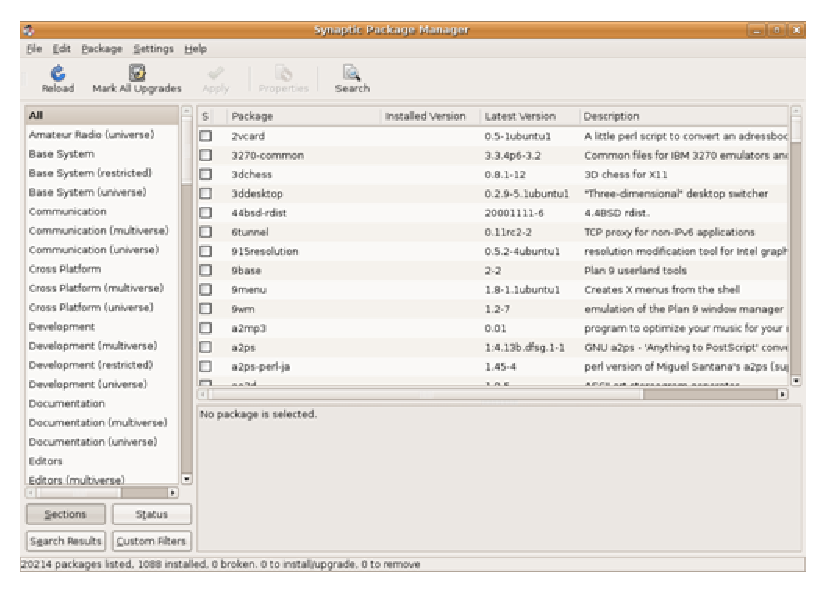
\includegraphics[scale=0.7]{figs/synaptic}
	\vspace{0.1in}
	\caption{Administrador de software Synaptic}
	\label{fig:synaptic}
\end{figure}

Para llevar a cabo este procedimiento se deben seguir los siguientes pasos:

% \begin{enumerate}
%   \item Abrir una consola e ir a un directorio adecuado para descargar el
%   c\'odigo fuente.
%   \item Ejecutar el siguiente comando para obtener el c\'odigo fuente del repositorio \emph{git}:\\
%   \verb|git clone http://gnuradio.org/git/gnuradio.git|. Esto crear\'a un nuevo
%   directorio llamado \emph{gnuradio}.
%   \item Entrar al nuevo directorio y ejecutar el siguiente comando:\\
%   \verb|./bootstrap|
%   \item Ejecutar el siguiente comando para configurar la instalaci\'on:\\
%   \verb|./configure|
%   \item Iniciar la compilaci\'on con el siguiente comando: \\
%   \verb|make|
%   \item Realizar una serie de pruebas para asegurar que la compilaci\'on fue
%   exitosa:\\
%   \verb|make check|
%   \item Instalar \emph{GNURadio}: \\
%   \verb|sudo make install|
% \end{enumerate}

\begin{enumerate}
  \item Color en alguna carpeta el archivo \emph{gnuradio-3.3.0.tar.gz} que se proporciona en el CD.
  \item Abrir una consola e ir a un directorio adecuado para descargar el
  c\'odigo fuente.
  \item Ejecutar el siguiente comando descomprimir el archivo \emph{tar}:\\
  \verb|tar xfz gnuradio-3.3.0.tar.gz|.
  \item Entrar al nuevo directorio \verb|gnuradio-3.3.0| y ejecutar el siguiente comando:\\
  \verb|./bootstrap|
  \item Ejecutar el siguiente comando para configurar la instalaci\'on:\\
  \verb|./configure|
  \item Iniciar la compilaci\'on con el siguiente comando: \\
  \verb|make|
  \item Realizar una serie de pruebas para asegurar que la compilaci\'on fue
  exitosa:\\
  \verb|make check|
  \item Instalar \emph{GNURadio}: \\
  \verb|sudo make install|
\end{enumerate}

De acuerdo a la documentaci\'on de \emph{GNURadio}, antes de realizar las
pruebas que verifican la compilaci\'on es necesario ejecutar la siguiente serie
de comandos:

\begin{enumerate}
  \item Copiar el archivo \emph{ld.so.conf} a un directorio temporal para
  modificarlo:\\
  \verb|cp /etc/ld.so.conf /tmp/ld.so.conf|
  \item Agregar la ruta donde est\'an instaladas las librer\'ias:\\
  \verb|echo /usr/local/lib >> /tmp/ld.so.conf|
  \item Borrar el archivo temporal y mover el nuevo a su lugar orignal:\\
  \verb|mv /tmp/ld.so.conf /etc/ld.so.conf|
  \item Ejecutar el siguiente comando para aplicar los cambios:\\
  \verb|sudo ldconfig|
\end{enumerate}

La raz\'on del procedimiento anterior es que \emph{Ubuntu} utiliza una
implementaci\'on diferente de la herramienta \emph{libtool} y si la ruta de las
librer\'ias no se especifica en el archivo de configuraci\'on, las pruebas
de \emph{GNURadio} fallan con errores de que no se encuentran dichas
librer\'ias \cite{radio}.


Para el uso \'optimo del USRP es necesario realizar una modificaci\'on en el
servicio \emph{udev} ya que \'unicamente permite acceso directo del dispositivo
a cuentas con privilegios de administrador. Esto quiere decir que cada que
se necesite ejecutar alg\'un programa que utilice el puerto USB es necesario
elevar el ejecutable con el comando \verb|sudo|. Para evitar esto se aplican los siguientes pasos:

\begin{enumerate}
  \item Crear un nuevo grupo de usuarios:\\
  \verb|sudo addgroup usrp|
  \item Anexar la cuenta de usuario que se est\'a utilizando a este nuevo
  grupo:\\
  \verb|sudo usermod -G usrp -a <CUENTA_DE_USUARIO>|
  \item Crear un archivo temporal con las instrucciones que \emph{udev} necesita
  para agregar este nuevo grupo a los que est\'an permitidos acceder al puerto
  USB:\\
  \verb|echo 'ACTION=="add", BUS=="usb", SYSFS{idVendor}=="fffe",|\\
  \verb|SYSFS{idProduct}=="0002", GROUP:="usrp", MODE:="0660"'|\\
  \verb|> tmpfile|
  \item Modificar los atributos de este archivo para que sea propiedad de root:\\
  \verb|sudo chown root.root tmpfile|
  \item Mover el archivo temporal al directorio de reglas de \emph{udev}:\\
  \verb|sudo mv tmpfile /etc/udev/rules.d/10-usrp.rules|
\end{enumerate}

Es posible aplicar los cambios al ejecutar el siguiente comando:\\
\verb|sudo udevadm control--reload-rules|. Si esto no funciona entonces se necesita reiniciar la PC
para que los cambios tengan efecto.

% Para poder actualizar el c\'odigo fuente con los cambios m\'as recientes del repositorio \emph{git}, se deben seguir los
% siguientes pasos:
% 
% \begin{enumerate}
%   \item Desinstalar la versi\'on actual con el siguiente comando: \verb|make uninstall|
%   \item Descargar las actualizaciones e integrarlas al c\'odigo fuente que ya se tiene con el siguiente comando:
%   \verb|git pull|. De esta manera no es necesario tener que descargar todo el c\'odigo fuente ya que \'unicamente se integraran
%   las diferencias entre el c\'odigo que ya se tiene y el que se encuentra en el repositorio.
%   \item Realizar los pasos para compilar el nuevo c\'odigo:
%   \begin{enumerate}
%     \item \verb|./bootstrap|
%     \item \verb|./configure|
%     \item \verb|make|
%     \item \verb|make check|
%     \item \verb|sudo make install|
%    \end{enumerate}
% \end{enumerate}
% 
% Si por el proceso de actualizaci\'on marca algun error del cual no se pueda recuperar, entonces es posible corregir
% el repositorio local (el c\'odigo fuente que se descarg\'o) sin tener que iniciar desde cero. Para
% lograr esto es necesario ejecutar el siguiente comando: \verb|git clean -d -x -f|. Este comando vuelve a establecer el repositorio a su
% estado original desde la \'ultima vez que se descarg\'o de la p\'agina de \emph{GNURadio}, aunque se debe tomar en cuenta que si
% se realizaron cambios en el c\'odigo fuente por parte del usuario, estos se van a perder. Una vez realizado esto se puede volver a
% intentar el proceso de actualizaci\'on.
